\documentclass[a4paper,12pt,twoside]{report}
\usepackage{fancyhdr}
\usepackage[utf8]{inputenc}
\usepackage[T1]{fontenc}
\usepackage[italian]{babel}
\usepackage{amsmath}
\usepackage{mathtools}
\usepackage{listings}
\usepackage{amssymb}
\usepackage{cancel}
\usepackage{tikz}
\usetikzlibrary{angles, quotes}
\usepackage{tikz-3dplot}
\usepackage{mathptmx}
\usepackage{tzplot}
\newcommand{\taninv}{\tan^{-1}}
\usepackage{titlesec}
\usepackage{algpseudocode}
\usepackage{multicol}
\usepackage{graphicx}

\graphicspath{ {./img/} }

\newcommand\pseudo[1]{\setlength\parindent{0pt}\texttt{#1}\setlength\parindent{24pt} \\}
\newcommand\hlin{\noindent\rule[0.5ex]{\linewidth}{1pt}}
\newcommand\take[2]{#1 $\leftarrow$ #2}

\newcommand\floor[1]{\left\lfloor#1\right\rfloor}
\newcommand\ceil[1]{\left\lceil#1\right\rceil}

\newcommand\insort{\texttt{INSERTION\_SORT }}
\newcommand\mergesort{\texttt{MERGE\_SORT }}
\newcommand\quicksort{\texttt{QUICK\_SORT }}
\newcommand\heapsort{\texttt{HEAP\_SORT }}

\titleformat{\chapter}
	{\Large\bfseries} 	% format
	{}							% label
	{0pt}						% sep
	{\huge}					% before-code
	 

\begin{document}
\title{Appunti del corso di Algoritmi 

A.A. 2023/2024}
\author{Prof. Roberto Segala \\ 
Appunti by Nick}
\date{}
\maketitle
\tableofcontents
% Aggiungere qui una eventuale introduzione come capitolo 0 (\chapter*{Introduzione} che spiega
% come usare queste note. 

\chapter{Introduzione}
% ================================= LEZIONE 1 =================================
\section{Problema dell'elemento minimo di un array}

\subsection{Trovare l'elemento minimo di un array - ragionamento intuitivo}
Prendiamo in esame l'algoritmo per trovare l'elemento minimo in un array di 
\emph{n} elementi cos\`{i} definito:

\hlin

\pseudo{n $\leftarrow$ LENGTH[A]}
\texttt{m $\leftarrow$ A[1] \\
FOR i $\leftarrow$ 1 TO n \\
\indent IF A[i] < m \\
\indent\indent m $\leftarrow$ A[i] \\
RET m
}

\hlin

Possiamo dire, in modo intuitivo, che il numero minimo di confronti da eseguire, per
esser certi di aver trovato il minimo elemento dell'array \`{e} $n-1$.

\subsection{Dimostrazione per assurdo}
Supponiamo ci venga detto che un algoritmo pu\`{o} trovare il minimo elemento di un
array in con meno di $n-1$ confronti. Se consideriamo i confronti fra gli elementi come
a delle \emph{gare} a coppie in cui `vince' l'elemento pi\`{u} piccolo tra i due, 
possiamo dire che il minimo elemento dovr\`{a} essere l'elemento che non ha perso 
nemmeno una gara.

Consideriamo l'array \textbf{A}, contenente gli elementi B e C, con B elemento minimo.
Se diamo come input all'algoritmo l'array \textbf{A}, otteniamo B come output, che 
\`{e} corretto. Ma sappiamo anche che C non ha mai perso una gara, quindi abbiamo due
elementi che non hanno mai perso una gara. Se ora modifichiamo C nel seguente modo 
$C = B-1$, otteniamo che C diventa l'elemento minimo, ma se applichiamo l'algoritmo 
all'array, otterremo ancora B come elemento minimo. 

Questo dimostra che \textbf{non \`{e} possibile} trovare il minimo di un array in meno di $n-1$ 
confronti.
% ================================= LEZIONE 2 =================================
\section{Compessit\`{a}}
\subsection{Concetto di Complessit\`{a}}
L'obiettivo dello studio degli algoritmi \`{e} quello di confrontare tra loro diversi 
algoritmi per determinare qualse sia il migliore caso per caso. Gli algoritmi possono
essere confrontati su vari criteri:
\begin{itemize}
\item costo di esecuzione (memoria, cpu, ...)
\item tempo di esecuzione
\item costo economico
\end{itemize}

Analizzeremo la \emph{complessit\`{a} legata al tempo di esecuzione}, ma la stessa
teoria \`{e} applicabile alla memoria o ad altri criteri di analisi degli algoritmi.

Il tempo di esecuzione pu\`{o} cambiare al variare della macchina su cui l'algoritmo 
viene eseguito; quindi, \`{e} inutile misurare il tempo fisico di completamento di un
algoritmo. Per determinarne la velocit\`{a} conteremo il numero di istruzioni, 
soprattutto quelle che hanno un impatto significativo sul tempo di esecuzione.

La \emph{complessit\`{a}} \`{e} dunque una funzione che prende in input la 
\emph{dimensione di un problema} e fornisce in output il tempo di esecuzione di un
algoritmo. Per sapere se la misura della dimensione del problema \`{e} corretta, lo
possiamo evincere dai dai risultati ottenuti. Ad esempio, se consideriamo una matrice, 
potremmo considerare come dimensione del problema il numero di elementi della matrice, 
oppure potremmo considerare come dimensione del problema $num. righe * num. colonne$.

\subsection{Alcuni esempi intuitivi}
Consideriamo un algoritmo come un insieme di blocchi $B_i$ di istruzioni messi in sequenza, e la complessit\`{a} $C_i(n)$ di ogni blocco:
\begin{center}
\begin{tabular}{c|c}
$B_1$ & $C_1(n)$ \\
$B_2$ & $C_2(n)$ \\
$B_3$ & $C_3(n)$ \\
\end{tabular}
\end{center}
Potremmo calcolare la complessit\`{a} di ogni blocco $C_i(n)$ e considerare la 
complessit\`{a} totale come la sommatoria delle complessit\`{a}:
\[ \sum_{i} C_i(n) \]

Ma se l'algoritmo presentasse delle condizioni, per esempio

\hlin

\pseudo{IF cond}
\texttt{\indent B\textsubscript{1} \\
ELSE \\
\indent B\textsubscript{2} \\
}
\hlin

\noindent allora la complessit\`{a} di un blocco condizionale diventerebbe $max(C_1(n), C_2(n))$.
In alcuni casi, inoltre, la complessit\`{a} della condizione dipende dal problema, ad 
esempio nel caso della ricorsione.

Analizziamo un altro algoritmo, contenente un ciclo:

\hlin

\pseudo{WHILE cond}
\texttt{\indent B}

\hlin

\noindent In questo caso, la complessit\`{a} sar\`{a} data dalla formula $C(B) * (numero interazioni)$. Non possiamo sapere a priori il numero di iterazioni, ma possiamo ricavare un limite superiore al numero di volte che il ciclo while viene eseguito.
\subsection{Limite inferiore, limite superiore}
Esistono molti modi che ci portano a sovrastimare il numero di istruzioni che viene 
eseguito. Il modo per capire se la previsione \`{e} accurata \`{e} quello di trovare
anche un \emph{limite inferiore}. Quanto pi\`{u} vicini saranno il limite superiore e
il limite inferiore, tanto pi\`{u} precisa \`{e} la previsione sulla complessit\`{a} 
dell'algoritmo. 
Qualunque sia la stima che facciamo, siamo obbligati a fare approssimazioni, per 
eccesso o per difetto. In questi casi \`{e} necessario avere un limite superiore e un 
limite inferiore del \emph{caso pessimo}. Non sarebbe utile calcolare il tempo medio, 
in quanto servirebbe una conoscenza probabilistica dell'input.

\subsection{Trovare il minimo elemento di un array}
Tornando sul problema della ricerca dell'elemento minimo di un array, proviamo a 
determinare la complessit\`{a} dell'algoritmo precedentemente scritto:

\hlin

\pseudo{n $\leftarrow$ LENGTH[A]\indent\indent// 1 istruzione} 
\texttt{m $\leftarrow$ A[1] \indent // 2 istruzioni \\
FOR i $\leftarrow$ 1 TO n \indent\indent // $4*(n-1)+1+2*(n-1)$ istr. \\
\indent IF A[i] < m \indent\indent // $2 + 2$ istr. (tutto il blocco if) \\
RET m \indent\indent // 1 istruzione \\
}
\hlin

Per come abbiamo contato le istruzioni necessarie per ogni riga dell'algoritmo, possiamo ottenere una formula di complessit\`{a} di questo tipo:
\[ 1+6*(n-1)+2+1+1 \]
Che possiamo semplificare in $6n-1$ e possiamo generalizzare, ignorando le costanti numeriche, in $an+b$, per qualche $a$ e qualche $b$.

\subsection{Confronto tra algoritmi}
Avendo due algoritmi con complessit\`{a} rispettivamente
\begin{itemize}
\item Alg. 1: $an+b$ 
\item Alg. 2: $an^2+bn+c$ 
\end{itemize}
conviene sempre scegliere l'Alg. 1, questo perch\'{e} se $n=1000$, nel caso dell'Alg. 1
stiamo moltiplicando la complessit\`{a} per $1000$, mentre nell'Alg. 2 la 
complessit\`{a} viene moltiplicata per $1000000$.

Quello che interessa, quindi, ai fini dell'analisi della complessit\`{a} di un 
algoritmo \`{e} il \emph{grado della funzione risultante}.

\subsection{Prodotto fra due matrici}
Analizziamo ora l'algoritmo che moltiplica due matrici:

\hlin

\pseudo{MULT(A,B)}
\texttt{\indent \take{n}{ROWS[A]} \\
\indent \take{m}{COLS[A]} \\
\indent \take{l}{COLS[B]} \\
\indent FOR \take{i}{1} TO n: \indent // costo $n*m*l*a$ \\
\indent\indent FOR \take{j}{1} TO l: \indent // costo $m*l*a$ \\
\indent\indent\indent \take{C[i][j]}{0} \\
\indent\indent\indent FOR \take{k}{1} TO m \indent // costo $m*a\cancel{+b}$ \\
\indent\indent\indent\indent \take{C[i][j]}{C[i][j] + A[i][j] * B[i][j]} \\
\indent RET C
}

\hlin

Possiamo notare che la complessit\`{a} del ciclo pi\`{u} interno \`{e} data da un
valore costante di istruzioni (riga 9) moltiplicato per il numero di iterazioni 
del ciclo ($m$), ottenendo quindi $m*a+b$, dove $b$ \`{e} il numero di istruzioni 
legate all'esecuzione del ciclo (verifica condizione, incremento indice, ecc).
Il ciclo centrale avr\`{a} una complessit\`{a} legata a $m*a$ eseguito $l$ volte, 
quindi otteniamo la formula $m*l*a$. Infine, il ciclo pi\`{u} esterno ha come complessit\`{a} la formula $n*m*l*a$, ottenuta in modo analogo alla precedente. Possiamo notare che il valore della costante $a$ non \`{e} di nostro interesse, ma la cosa importante \`{e} che la complessit\`{a} dell'algoritmo \`{e} lineare in $n$, $l$ ed $m$.

\chapter{Notazione asintotica}
% ================================= LEZIONE 3 =================================
\section{Notazione asintotica}
Dalle funzioni di complessit\`{a} ci interessa principalmente ricavare l'ordine di grandezza; ad esempio \`{e} importante sapere se al raddoppio della dimensionde del problema il tempo di completamento raddoppia oppure quadruplica.
In alcuni casi il problema potrebbe avere complessit\`{a} diverse sulla base di 
eventuali condizioni che si verificano durante l'esecuzione, ad esempio se viene eseguito il ramo \texttt{if} o il ramo \texttt{else}. In questi casi dobbiamo considerare il caso pessimo. \\
\textbf{Esempio:} la ricerca di un elemento in un array costa $n$, ma esiste 
un caso in cui costa $1$, ovvero quando l'elemento che si sta cercando \`{e} il primo.

\subsection{O-grande - $f \in O(g)$}
Diciamo che una funzione $f$ appartiene ad O-grande di g, $f \in O(g)$, quando $f$ non cresce pi\`{u} in fretta di $g$ da un certo punto in poi, a prescindere dalle costanti.
\subsubsection{Definizione:}
\[ \exists c>0 \thickspace \exists \bar{n}>0 \thickspace \forall n>\bar{n} \thickspace f(n) \le cg(n) \]
\subsubsection{Grafico:}
\begin{tikzpicture}
\draw[->] (0,-1) -- (0,3) node[above]{y};
\draw[->] (-1,0) -- (12,0) node[right]{x};
\draw[teal][line width=0.5mm] plot [smooth, tension=1] coordinates { %
	(1,-1) (4.5,0.5) (6.8,2.3)
	}node[above right] {$g(n)$};
\draw[blue][line width=0.5mm] plot [smooth, tension=1] coordinates { %
	(-0.5,-0.5) (3.5,1) (5.9,2.6) 
	} node[above right] {$f(n)$};
\draw[red][line width=0.5mm] plot [smooth, tension=1] coordinates { %
	(1,-0.7) (3.5, 1.2) (5.1, 3)
	} node[above right] {$cg(n)$}; 
\node at (0,0) [below left] {$O$};
\draw[dashed] (3,0.75) -- (3,-0.55) node[below] {$\bar{n}$};
\filldraw[black] (3,0.75) circle (2pt);
\end{tikzpicture}
\subsection{Omega - $f \in \Omega(g)$}
Diciamo che una funzione $f$ appartiene ad Omega di g, $f \in \Omega(g)$, quando da un certo punto in poi, a meno di una costante moltiplicativa, $f$ non va mai al di sotto di $g$.
\subsubsection{Definizione:}
\[ \exists c>0 \thickspace \exists \bar{n} > 0 \thickspace \forall n > \bar{n} \thickspace f(n) \ge cg(n) \]
\subsubsection{Grafico:}
\begin{tikzpicture}
\draw[->] (0,-1) -- (0,3) node[above]{y};
\draw[->] (-1,0) -- (12,0) node[right]{x};
\draw[red][line width=0.5mm] plot [smooth, tension=1] coordinates { %
	(-1,-0.2) (2.8,0.5) (6.8,2.3)
	}node[above right] {$cg(n)$};
\draw[blue][line width=0.5mm] plot [smooth, tension=1] coordinates { %
	(-0.5,-0.5) (3.5,1) (5.9,2.6) 
	} node[above right] {$f(n)$};
\draw[teal][line width=0.5mm] plot [smooth, tension=1] coordinates { %
	(-1,0.2) (2.8, 1.4) (5.1, 3)
	} node[above right] {$g(n)$}; 
\node at (0,0) [below left] {$O$};
\draw[dashed] (1.4,0.15) -- (1.4,-0.2) node[below] {$\bar{n}$};
\filldraw[black] (1.4,0.15) circle (2pt);
\end{tikzpicture}
\subsection{Theta - $f \in \Theta(g)$}
Una funzione $f$ appartiene a Theta di $g$ se e solo se $f$ appartiene ad O-grande di $g$ ed $f$ appartiene a Omega di $g$. Formalmente scriviamo:
\[ f \in \Theta(g) \leftrightarrow f \in O(g) \and f \in \Omega(g) \]
\subsection{Esercizio}
Dimostrare che $f \in O(g) \leftrightarrow g \in \Omega(f)$
\paragraph{Dimostrazione:}
\begin{itemize}
\item Dimostriamo l'implicazione a destra: $f \in O(g) \rightarrow g \in \Omega(f)$. Usiamo la definizione: 
\[ \exists c \thickspace \exists \bar{n} \thickspace \forall n > \bar{n} \thickspace f(n) \le cg(n) \]
Siano $c$ ed $\bar{n}$ due valori che soddisfano la formula $\forall n>\bar{n} \thickspace f(n) \le cg(n)$. Vogliamo dimostrare che vale 
\[ \exists c' \thickspace \exists \bar{n}' \thickspace \forall n > \bar{n}' \thickspace g(n) \ge c' f(n) \] 
quindi \[f(n) \le cg(n)\]
\[ \frac{1}{c}f(n) \le g(n) \]
\[ g(n) \ge \frac{1}{c}f(n) \]
Fissiamo $c'=\frac{1}{c}$ e otteniamo che:
\[ g(n) \ge c'f(n) \]
$\forall n > \bar{n}$, con $\bar{n}' = \bar{n}$.
\item Dimostriamo l'implicazione a sinistra: $g \in \Omega(f) \rightarrow f \in O(g)$
\[ \exists c \thickspace \exists \bar{n} \thickspace \forall n > \bar{n} \thickspace g(n) \ge cf(n) \]
Siano $c$ ed $\bar{n}$ due valori che soddisfano la formula $\forall n > \bar{n} \thickspace g(n) \ge cf(n)$. Vogliamo dimostrare che vale
\[ \exists c'' \thickspace \exists \bar{n}'' \thickspace \forall n > \bar{n}'' \thickspace f(n) \le c''g(n) \]
quindi
\[ g(n) \ge cf(n) \]
\[ \frac{1}{c} g(n) \ge f(n) \]
\[ f(n) \le \frac{1}{c} g(n) \]
Fissiamo $c''=\frac{1}{c}$ e otteniamo che:
\[ f(n) \le c''g(n) \]
$\forall n > \bar{n}$, con $\bar{n}'' = \bar{n}$.
\end{itemize}
\begin{flushright}$\square$\end{flushright}

\subsection{Notazione di uso comune}
Sia $A$ un algoritmo. 
\begin{itemize}
\item Affermare che $A \in O(f)$ significa che $\exists g \in O(f)$ tale che $A$ \emph{termina sempre entro tempo g}.
\item Affermare che $A \in \Omega(f)$ significa che \emph{esiste uno schema di input} tale che su quello schema $A$ richiede almeno $g$ operazioni con $g \in \Omega(f)$.
\item Se combaciano allora diciamo che $A \in \Theta(f)$.
\end{itemize}
Sia $P$ un problema.
\begin{itemize}
\item Dire che $P \in O(f)$ significa che $\exists A$ che risolve $P$, con $A \in O(f)$.
\item Dire che $P \in \Omega(f)$ significa che $forall A$ che risolve $P$, con $A \in \Omega (f)$.
\item Se combaciano diciamo che $P \in \Theta (f)$.
\end{itemize}

\subsection {Equazioni di ricorrenza}
\subsubsection{Calcolo del fattoriale di un numero}
\pseudo{FATT(n)}
\indent \texttt{IF n = 0 THEN \\
\indent\indent RET 1 \\
\indent ELSE \\
\indent\indent RET n * FATT(n-1) \\
}
L'equazione di ricorrenza corrispondente \`{e}:
\begin{equation}
T(n) = 
\begin{cases}
c & \text{se $n = 0$}\\ 
1 + T(n-1) & \text{se $n > 0$}
\end{cases}
\end{equation}

% ================================= LEZIONE 4 =================================
\section{Risoluzione di e quazioni di ricorrenza}
\subsection{Risoluzione di equazioni di ricorrenza - Metodo iterativo}
Prendendo in considerazione l'equazione di ricorrenza del fattoriale:
\begin{equation}
T(n) = 
\begin{cases}
c & \text{se $n = 0$} \\
1 + T(n-1) & \text{se $n > 0$}
\end{cases}
\end{equation}
Possiamo risolvere l'equazione come segue:
\[ T(n) = 1 + T(n-1) \]
\[ = 1 + (1 + T(n-2)) \]
\[ = 2 + T(n-2) \]
\[ = 2 + (1 + T(n-3)) \]
\[ = \dots = i + T(n-i) \]
\[= \dots = n + t(n-n) = n + 1 \]
Questa serie di passaggi intuitivi possono essere verificati per induzione.
\subsubsection{Esempio di risoluzione con metodo iterativo}
Data l'equazione $ T(n) = 3T(\floor{\frac{n}{4}}) + n $, applichiamo il metodo
iterativo per risolverla.
\[= 3\left(3T\left(\floor{\frac{\floor{\frac{n}{4}}}{4}} \right)+\floor{\frac{n}{4}}\right) + n\]
\[ = 3\left(3T\left(\floor{\frac{n}{4^2}}\right) + \floor{\frac{n}{4}}\right) + n \]
\[ = 3^2 T\left(\floor{\frac{n}{4^2}}\right) + 3 \floor{\frac{n}{4}} + n \]
\[ = 3^2\left(3T\left(\floor{\frac{\floor{\frac{n}{4^2}}}{4}}\right) + \floor{\frac{n}{4^2}}\right) + 3 \floor{\frac{n}{4}} + n \]
\[ = 3^3T\left( \floor{\frac{n}{4^3}}\right) + 3^2\floor{\frac{n}{4^2}} + 3\floor{\frac{n}{4}} + n \]
Dopo $i$ iterazioni otteniamo:
\[ 3^i T\left(\floor{\frac{n}{4^i}}\right)+3^{i-1}\floor{\frac{n}{4^{i-1}}} + 3^{i-2} \floor{\frac{n}{4^{i-2}}} + \dots + 3\floor{\frac{n}{4}} + n \]
\[ = 3^{i} T\left(\floor{\frac{n}{4^{i}}}\right) + \left(\sum_{k=1}^{i-1} 3^k \floor{\frac{n}{4^k}} \right) + n \]


Se $4^i \ge n \rightarrow i \ge log_{4}{n}$ sono sicuramente in un caso base.
\newline
Otteniamo:
\[ = 3^{log_{4}{n}} T\left(\floor{\frac{n}{4^{log_{4}{n}}}}\right) + \left(\sum_{k=1}^{log_{4}{n}-1} 3^k \floor{\frac{n}{4^k}} \right) + n \]

Quando siamo nel caso base possiamo dire che $T\left(\floor{\frac{n}{4^{log_{4}{n}}}}\right)$ \`{e} una costante, quindi la sostituiamo con $c$.

\[ c3^{log_{4}{n}} + \left(\sum_{k=1}^{log_4{n-1}} 3^k \floor{\frac{n}{4^k}} \right) + n \]
Ora consideriamo $n = \left(\frac{3}{4}\right)^0 n$:
\[ \le c3^{log_{4}{n}} + \sum_{k=1}^{log_4{n-1}} 3^k \floor{\frac{n}{4^k}} + \left(\frac{3}{4}\right)^0n \]
\[ = c3^{log_{4}{n}} + \sum_{k=0}^{log_4{n-1}} 3^k \left(\frac{3}{4}\right)^kn \]
La costante $c$ non \`{e} rilevante, quindi possiamo eliminarla. Possiamo inoltre notare che $\sum_{k=0}^{log_{4}{n-1}} \left(\frac{3}{4}\right)^kn$ \`{e} una somma parziale di una serie geometrica di ragione $\frac{3}{4}$. Perci\`{o} possiamo dire che 
\[n \sum_{k=0}^{log_{4}{n-1}} \left(\frac{3}{4}\right)^k \le n\sum_{k=0}^{\infty} \left(\frac{3}{4}\right)^k = \Theta(n) \text{\emph{ \thickspace (lineare)}}\]
Ora dobbiamo analizzare l'altra parte della formula, ovvero $3^{log_{4}n}$
\[ 3^{log_{4}n} = n^{log_n3^{log_4n}} \]
\[\footnote[1]{formula del cambio di base del logaritmo.} = n^{log_4n * log_n3}\]
\[ = n^{log_43} \]
Otteniamo 
\[ T(n) = n^{log_43} + \Theta(n) \]
Quindi la soluzione dell'equazione di ricorrenza \`{e} $\Theta(n)$.

\subsection{Risoluzione di equazioni di ricorrenza - Metodo di sostituzione}
Data un'ipotesi andiamo a verificare se \`{e} corretta, sostituendo tutte le ocorrenze di $T(n)$ sulla destra con l'ipotesi da verificare.

\subsubsection{Esempio di risoluzione con metodo di sostituzione}

Data l'equazione di ricorrenza $T(n) = 2T\left(\floor{\frac{2}{n}}\right) + n$. Supponiamo ci venga detto che $T(n) \in O(nlogn)$.

Sostituiamo le ocorrenze di destra con la nostra ipotesi:
\[ T(n) \le 2 * c *\floor{\frac{n}{2}}log\floor{\frac{n}{2}} + n\]
\[ \le \cancel{2}* c* \frac{n}{\cancel{2}} \log \frac{n}{2} + n\]
(scegliamo per il logaritmo la base che ci fa comodo)
\[ \le cnlogn - cnlog_22 + n \]
\[ \le cnlogn - (cn -n) \le cnlogn \]
quando $(cn - n) \ge 0$, ovvero:
\[ n(c-1) \ge 0 \]
\[ \forall c \ge 1, \thickspace \bar{n} = \text{qualsiasi} \]
\paragraph{Nota:} se applicando il metodo di sostituzione, sostituendo l'ipotesi si ottiene l'ipotesi, allora abbiamo verificato che la nostra ipotesi \`{e} vera.
\subsection{Teorema dell'esperto - Master Theorem}
Questo teorema permette di risolvere tutte le equazioni di ricorrenza nella forma
\[ T(n) = aT(\frac{n}{b}) + f(n), \thickspace \text{ con $a \ge 1$, $b > 1$} \]
Il teorema prevede di confrontare l'ordine di grandezza di due funzioni ricavate dala formula precedente. Le due formule sono: 
\begin{itemize}
\item $f(n)$
\item $n^{log_ba}$
\end{itemize}
Il teorema prevede tre casi:
\begin{enumerate}
\item Se $f(n) \in O(n^{log_ba - \varepsilon})$, con $\varepsilon > 0$ allora $T(n) \in \Theta(n^{log_ba})$
\item Se $f(n) \in \Theta(n^{log_ba})$, allora $T(n) \in \Theta(f(n) log n)$
\item Se $f(n) \in \Omega(n^{log_ba + \varepsilon}$, con $\varepsilon > 0$, allora $T(n) \in \Theta(f(n))$, con $a f(\frac{n}{b}) \le c f(n)$, con $c < 1$ e $n > \bar{n}$.
\end{enumerate}
\subsubsection{Esempi}
\paragraph{Caso 1:} 
\[T(n) = 9T(\frac{n}{3}) + n\]
Ricaviamo le due funzioni da confrontare: $f(n) = n$ e $n^{log_ba} = n^{log_39} = n^{2}$. Siccome $n \in O(n^2)$ cerchiamo un $\varepsilon > 0$ tale che $n \in O(n^{2-\varepsilon})$. Prendendo $\varepsilon = 0.1$ \`{e} verificato il caso 1:
\[ \frac{n^2}{n^{0.1}} \to n \in O(n^{2-0.1})\]
\paragraph{Caso 2:}
\[ T(n) = T(\frac{2n}{3}) + 1 \]
Scomponiamo l'equazione di ricorrenza nei suoi componenti, come da teorema, e otteniamo $a = 1$, $b = \frac{2}{3}$ e la funzione nota $f(n) = 1$. 
Ora abbiamo che $n^{log_ba} = n^{log_{\frac{2}{3}1}} = 1$. Si pu\`{o} notare che $f(n) \in \Theta(n^1)$ e quindi siamo nel caso 2. 
\[ T(n) \in \Theta(f(n)logn) = \Theta(1logn)\]
\paragraph{Caso 3:}
\[T(n) = 3T(\frac{n}{4}) + nlogn \]
In questo caso abbiamo $a = 3$, $b = 4$ e $f(n) = nlogn$. $n^{log_43} < 1$, mentre $nlogn > 1$. Dobbiamo trovare un $\varepsilon$ tale che $(n^{log_43} * n^{\varepsilon}) < nlogn$. 
Graficamente possiamo notare che quasiasi $\varepsilon$ compreso tra $log_43$ e $1$, soddisfa la condizione:
\begin{center}
\begin{tikzpicture}
\draw (0,0) -- (2,0);
\draw (0,0.25) -- (0, -0.25);
\node at (0,-0.25) [below]{$log_43$};
\draw (2,0.25) -- (2, -0.25);
\node at (2,-0.25) [below]{$1$};
\draw[red] (1,0.25) -- (1, -0.25);
\node[red] at (1, -0.25) [below]{$\varepsilon$};
\end{tikzpicture}
\end{center}
Quindi possiamo prendere come $\varepsilon = \frac{1 - log_43}{2}$.
Essendo nel caso 3, dobbiamo verificare anche la condizione $af(\frac{n}{b}) \le c f(n)$:
\[\footnote[1]{se $a > b$, $c$ deve essere maggiore di 1, quindi non verifica la condizione.}  a\frac{n}{b}log\frac{n}{b} \le c (n log n), \thickspace \text{ c < 1} \]
\[ \frac{3}{4}n log \frac{n}{4} \le c(n log n), \thickspace \text{ c < 1} \]
con $c = \frac{3}{4}$ la condizione \`{e} soddisfatta. 

\paragraph{Caso 4: non \`{e} possibile applicare il teorema}
\[ T(n) = 2T(\frac{n}{2}) + n log n \]
Provando ad applicare il teorema a questa formula ricaviamo che $n^{log_22} = n^1$ e che la funzione nota $f(n) = n log n$. Dovremmo trovare un $\varepsilon > 0$ tale che $n log n \in (n - n^{\varepsilon})$, che \textbf{non esiste}.
In questo caso il teorema non \`{e} applicabile, ma potrebbe essere corretta la supposizione intuitiva che l'equazione di ricorrenza data appartenga ad uno dei tre casi. Per verificare se l'intuizione \`{e} corretta possiamo applicare il \emph{metodo di sostituzione}.


\chapter{Problema dell'ordinamento}
% ================================= LEZIONE 5 =================================
\section{Input, output e relazioni di ordinamento}
\paragraph{Input:} \`{e} definito come una sequenza di oggetti $a_1, \dots, a_n$ su cui \`{e} definita una relazione di ordinamento totale.
\paragraph{Output:} \`{e} una permutazione $a_{1}', \dots, a_{n}'$ di $a_1, \dots, a_n$ tale che per ogni $i < j$ si ha $a_{i}' \le a_{j}'$.
\paragraph{Relazione di ordinamento:} significa che esiste un metodo per determinare, dati due oggetti, quale sia il pi\`{u} piccolo e quale il pi\`{u} grande. Se non si conosce la \emph{relazione d'ordine}, senza confronti non siamo in grado di dire come due oggetti vanno ordinati tra loro, quindi l'unico modo che abbiamo per ordinare due oggetti \`{e} quello di confrontarli tra loro. 

\paragraph{Nota:} il problema dell'ordinamento $\in O(n^2)$. Inoltre, il problema dell'ordinamento $\in \Omega(n)$.

\newpage
\section{Insertion sort}
\subsection{Pseudocodice}

\hlin

\pseudo{INSERTION\_SORT(A)}
\texttt{\indent FOR j $\leftarrow$ 2 TO length(A) \\
\indent\indent key $\leftarrow$ A[j] \\
\indent\indent i $\leftarrow$ j - 1 \\
\indent\indent WHILE i $>$ 0 AND A[i] > key \\
\indent\indent\indent A[i+1] $\leftarrow$ A[i] \\
\indent\indent\indent \take{i}{i-1} \\
\indent\indent A[i+1] $\leftarrow$ key \\
}
\hlin

L'algoritmo \insort se applicato ad un array con elementi uguali, \emph{non scambia l'ordine relativo di tali elementi}, questo significa che \`{e} \textbf{stabile}. Inoltre, analizzando \emph{la quantit\`{a} di memoria si pu\`{o} vedere che \`{e} costante e non dipende dalla dimensione del problema}, questa propriet\`{a} significa che l'algoritmo \textbf{ordina in loco}.

\subsection{Complessit\`{a} di \insort}

Per calcolare la complessit\`{a} di \insort possiamo notare che il blocco \texttt{WHILE} viene eseguito \emph{al pi\`{u}} $n$ volte, il ciclo \texttt{FOR} viene ripetuto $(n-1)$ volte. Come limite superiore, intuitivamente, abbiamo $n^2$, ma potrebbe essere una stima esagerata. Alla prima iterazione fa al massimo 1 confronto, alla seconda iterazione fa 2 confronti e se arriviamo all'ultima iterazione i confronti sono $n\cancel{-1}$\footnote[1]{Non ci interessano le costanti, possiamo togliere il $-1$ e approssimare a $n$.}. 

Possiamo quindi formulare la complessit\`{a} di \insort nella formula
\[1 + 2 + 3 + \dots + n = \frac{n(n+1)}{2} \]
Concludendo che $\frac{n(n+1)}{2} \in \Theta(n^2)$.

\insort \`{e} un algoritmo a complessit\`{a} quadratica, ma in alcuni casi \`{e} molto veloce: se consideriamo un array di piccole dimensioni oppure un array quasi completamente ordinato, l'algoritmo termina in tempo lineare. 

% ================================= LEZIONE 6 =================================
\section{Merge sort}
\subsection{Pseudocodice}

\hlin

\pseudo{MERGE\_SORT(A, p, r)} 
\texttt{\indent IF p < r \indent // quando p = r, l'array \`{e} ordinato \\
\indent\indent \take{q}{(p + r) / 2} \indent // implicita l'appross. per difetto \\
\indent\indent MERGE\_SORT(A, p, q) \indent // ordino la prima parte \\
\indent\indent MERGE\_SORT(A, q+1, r) \indent // ordino la seconda parte \\
\indent\indent MERGE(A, p, q, r)	\indent // unisco le due parti ordinate \\
}
\hlin

\hlin

\pseudo{MERGE(A, p, q, r)}
\texttt{\indent \take{i}{1} \indent // array risultato \\
\indent \take{j}{p}
\indent \take{k}{q+1}
\indent WHILE j <= q || k <=r \\
\indent\indent IF j <= q \&\& (k > r || A[j] <= A[k]) \indent // stabile \\
\indent\indent\indent \take{B[i]}{A[j]} \\
\indent\indent\indent \take{j}{j+1} \\
\indent\indent ELSE \\
\indent\indent\indent \take{B[i]}{A[k]}
\indent\indent\indent \take{k}{k+1} \\
\indent\indent \take{i}{i+1} \\
\indent FOR \take{i}{1} TO r - p + 1 \\
\indent\indent \take{A[i+p-1]}{B[i]} \\
}

\hlin

Salta subito all'occhio che \mergesort non ordina in loco, infatti nella \texttt{MERGE} si usa un array ausiliario $B$, ma la stabilit\`{a} \`{e} preservata. 

\subsection{Complessit\`{a} di \mergesort}

\mergesort \`{e} un algoritmo ricorsivo che agisce, ad ogni nuova chiamata, su un sotto array di dimensione $\frac{1}{2}$ rispetto all'array. La sua equazione di ricorrenza \`{e}:
\[ T(n) = 2T(\frac{n}{2}) + n \]
Siamo nel secondo caso indicato dal \emph{Master Theorem}, ovvero $T(n) \in \Theta(n log n)$.

\subsubsection{Esempio}
Consideriamo di dover ordinare 1 milione di dati, e abbiamo due opzioni:
\begin{enumerate}
\item Utilizziamo \insort su un supercomputer in grado di svolgere 100 milioni di istruzioni al secondo, con implementazione ottimizzata.  Complessit\`{a} calcolata $2n^2$.
\item Utilizziamo \mergesort su un PC ordinario in grado di svolgere 1 milione di istruzioni al secondo, con implementazione scarsa. Complessit\`{a} calcolata $50n log n$.
\end{enumerate}
Calcoliamo il tempo di esecuzione dell'algoritmo per verificare in quale contesto il tempo richiesto per risolvere il problema \`{e} minore. Nel caso 1 abbiamo
\[ t = \frac{2(10^6)^2}{10^8} = 20000 s = 5.56 h \]
Nel caso 2 abbiamo
\[ t = \frac{50 * 10^6 * 20}{10^6} = 1000 s = 16.67 min \]

Possiamo notare come le costanti siano poco influenti rispetto all'ordine di grandezza.
% ================================= LEZIONE 7 =================================
\newpage
\section{Quick sort}
\subsection{Pseudocodice}
\hlin

\pseudo{QUICK\_SORT(A, p, r)} 
\texttt{\indent IF p < r 
\indent\indent \take{q}{PARTITION(A, p, r)} \\
\indent\indent QUICK\_SORT(A, p, q) \\
\indent\indent QUICK\_SORT(A, q+1, r) \\
}
\hlin

\hlin

\pseudo{PARTITION(A, p, r)}
\texttt{\indent \take{x}{A[p]} \\
\indent \take{i}{p-1} \\
\indent \take{j}{r+1} \\
\indent WHILE TRUE \\
\indent\indent REPEAT \take{j}{j-1} \\
\indent\indent UNTIL A[j] <= x \\
\indent\indent REPEAT \take{i}{i+1} \\
\indent\indent UNTIL A[i] >= x \\
\indent\indent IF i < j \\
\indent\indent\indent SCAMBIA (A[i], A[j]) \\
\indent\indent ELSE \\
\indent\indent\indent RETURN j
}

\hlin

\quicksort non \`{e} stabile perch\'{e} la partition scambia gli elementi uguali,  ma ordina in loco. 

\subsection{Complessit\`{a} di \quicksort}

Il caso pessimo di \quicksort \`{e} un array ordinato. Possiamo intuitivamente scrivere un'equazione di ricorrenza per \quicksort cosi:
\[ T(n) = C(partition) + T(1) + T(n-1) \]
Analizzando \texttt{PARTITION} si nota che la sua complessit\`{a} \`{e} lineare, perch\`{e} deve svolgere al pi\`{u} $n$ operazioni, $\frac{n}{2}$ nel primo \texttt{REPEAT-UNTIL} ed $\frac{n}{2}$ nel secondo. 
Otteniamo quindi l'equazione
\[ T(n) = n + T(n-1) = \frac{n(n+1)}{2} \Rightarrow T(n) \in \Theta(n^2) \]
quindi la complessit\`{a} di \quicksort \`{e} quadratica.

Si nota anche che, nel caso medio, quando l'array \`{e} totalmente disordinato, l'algoritmo \`{e} lineare. Se troviamo quindi un modo per prendere la \texttt{x} della partition in modo casuale, ed avendo casi d'uso in cui l'algoritmo \`{e} utilizzato molte volte, possiamo avvicinarci al caso medio sempre di pi\`{u}.

\hlin

\pseudo{RANDOMIZED\_PARTITION(A, p, r)}
\texttt{\indent i <- RANDOM (p, r) \\
\indent SCAMBIA (A[i], A[p]) \\
\indent RETURN PARTITION (A, p, r) 
}

\hlin

A questo punto $T(n)$ non \`{e} pi\`{u} definito ma casuale, e abbiamo uno spazio campione di tutte le possibili esecuzioni dell'algoritmo. Per ogni esecuzione sappiamo quanto tempo richiede:
\[ T(n) = n + \frac{1}{n}(T(1)) + T(n-1) + \frac{1}{n}(T(2) + T(n-2) + \dots + \frac{1}{n}(T(n-1)+ T(1)) \]
\[ = n + \frac{1}{n} \sum_{i=1}^{n-1}(T(i) + T(n-i)) = n + \frac{2}{n}\sum_{i=1}^{n-1} T(i) \]
E otteniamo che $T(n) \le n log n$.

\subsection{Rimozione della ricorsione di coda}

Analizzando la complessit\`{a} di \quicksort rispetto alla memoria notiamo che lo stack di attivazione pu\`{o} crescere molto a causa delle chiamate ricorsive. Possiamo ridurle sostituendo l'ultima con un ciclo:

\hlin

\pseudo{QUICK\_SORT(A, p, r)}
\texttt{\indent WHILE p < r \\
\indent\indent \take{q}{PARTITION(A, p, r)} \\
\indent\indent QUICK\_SORT(A, p, q) \\
\indent\indent \take{p}{q+1} \\
}

\hlin

Se ora si riuscisse a trasformare questo algoritmo in modo tale da eseguire la chiamata ricorsiva sul sottoarray pi\`{u} piccolo tra i due generati dalla partition, ridurremmo ulteriormente lo stack di attivazione.

\section{Struttura dati: Heap}
Lo heap \`{e} una struttura dati ad albero binario, divisibile in livelli. Ogni livello contiene dei nodi, se un nodo non ha figli viene detto foglia. Quando un livello, partendo da sinistra, non ha tutti i nodi, si dice che il livello \`{e} semicompleto. Un albero che come ultimo livello ha un livello semicompleto, si dice albero semicompleto. Naturalmente, un albero che presenta tutti i nodi anche sull'ultimo livello si dice completo.
\begin{multicols}{2}
\textbf{Albero completo}

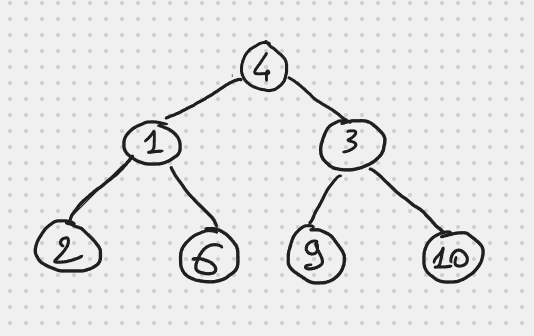
\includegraphics[scale=0.3]{alberocompleto}

\textbf{Albero semicompleto}

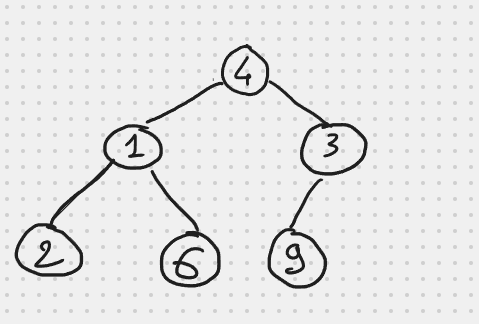
\includegraphics[scale=0.3]{alberosemicompleto}
\end{multicols}
\subsection{Rappresentazione di un albero come array}
Gli alberi binari semicompleti possono essere rappresentati come un array. Prendendo un qualsiasi nodo, dividendone il suo indice per $2$ si ottiene l'indice del nodo genitore, mentre per ottenere gli indici dei figli basta prendere l'indice del genitore e moltiplicarlo per $2$ per il figlio sinistro, e sommare $1$ per il figlio destro.
\begin{center}
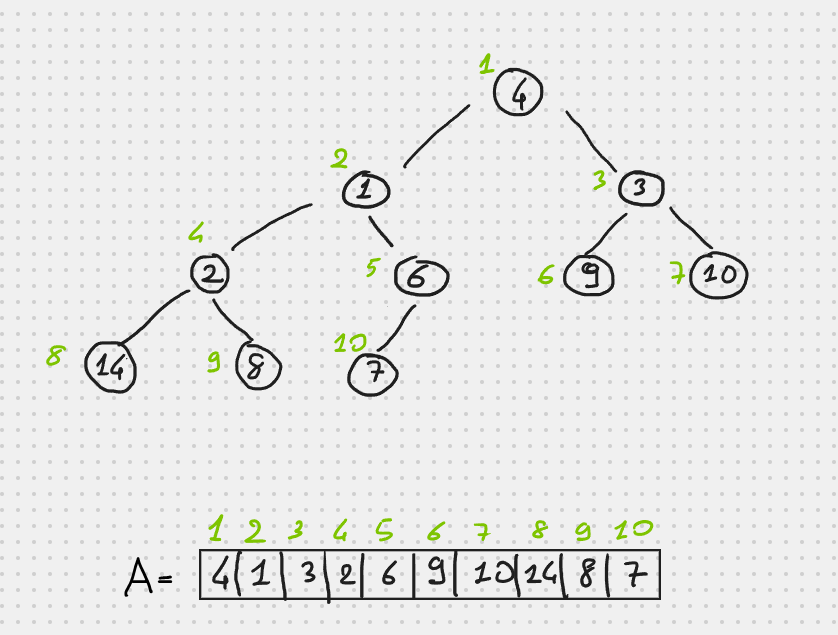
\includegraphics[scale=0.55]{albero2array}
\end{center}
Per esempio, se il nodo con valore 4 ha indice $1$, il figlio sinistro, nodo di valore $1$ sar\`{a} \texttt{A[1*2]}, mentre il figlio destro (nodo di valore 6) \texttt{A[(1*2)+1]}.
\begin{center}
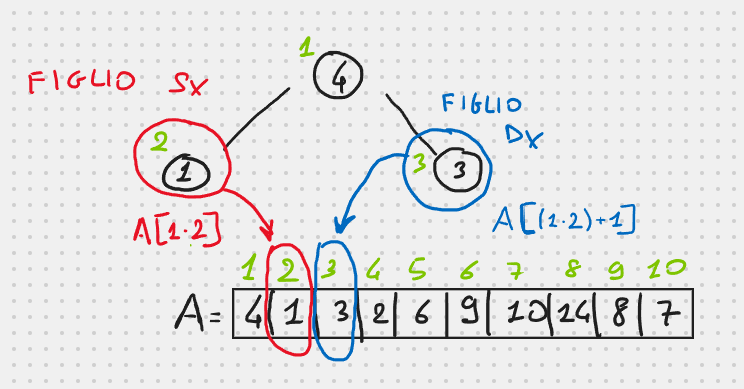
\includegraphics[scale = 0.6]{esempioa2a}
\end{center}

\subsection{Heap}

Come ulteriore vincolo, perch\'{e} un albero sia uno heap, dobbiamo imporre che gli oggetti che fanno parte dell'albero devono avere una relazione di ordinamento tra loro e i figli devono essere minori o uguali del nodo genitore. In uno heap completo con $h$ livelli ci sono $log_2h$ nodi.
\[ 2^0 + 2^1 + 2^3 + \dots + 2^h = 2^{h+1} -1 \]
\[n \ge 2^h \Rightarrow log n \ge h \]
In questo modo ho la garanzia che nello heap l'elemento pi\`{u} grande, o il pi\`{u} piccolo se cambio la relazione di ordinamento, lo trovo alla radice. Quindi in uno heap memorizzato in un array, l'elemento di indice $1$ sar\`{a} il massimo (o il minimo).
\newpage

\section{Heap sort}

Utilizzando lo heap possiamo creare un algoritmo di ordinamento:

\hlin

\pseudo{HEAPIFY(A, i)}
\texttt{\indent \take{l}{LEFT(i)} \indent // ret. indice figlio sx \\
\indent \take{r}{RIGHT(i)} \indent // ret. indice figlio dx \\ 
\indent IF l <= HEAPSIZE(A) AND A[l] > A[i] \\
\indent\indent \take{largest}{l}	\indent // se figlio sx > genitore \\
\indent ELSE  \\
\indent\indent \take{largest}{i} \indent // se genitore > figlio sx \\
\indent IF r <= HEAPSIZE(A) AND A[r] > A[largest] \\
\indent\indent \take{largest}{r} \indent // se figlio dx > A[largest] \\
\indent IF i != largest \indent // se il genitore non \`{e} il maggiore \\
\indent\indent SCAMBIA (A[i], A[largest]) \indent // scambio il genitore con il maggiore dei figli\\
\indent\indent HEAPIFY (A, largest) \\ 
}

\hlin

\hlin 

\pseudo{BUILD\_HEAP(A)}
\texttt{\indent \take{HEAPSIZE(A)}{LENGTH(A)} \\
\indent FOR \take{i}{LENGTH(A) / 2} DOWNTO 1 \\
\indent\indent HEAPIFY(A, i) \\
}

\hlin

\hlin

\pseudo{HEAP\_SORT(A)} 
\texttt{\indent BUILD\_HEAP (A) \\
\indent FOR \take{i}{LENGTH(A)} DOWNTO 2 \\
\indent \indent SCAMBIA(A[1], A[i]) \\
\indent\indent \take{HEAPSIZE(A)}{HEAPSIZE(A) - 1} \\
\indent\indent HEAPIFY(A, 1)
}

\hlin

\heapsort ordina in loco, ma non \`{e} stabile.
\newpage
\subsection{Complessit\`{a} di \heapsort}

La complessit\`{a} massima di \texttt{HEAPIFY} \`{e} la profondit\`{a} massima dell'albero, ovvero $log n$ (dove $n$ \`{e} il numero di nodi).
In uno heap di $n$ nodi ci sono $\frac{n}{2}$ foglie al massimo. Perci\`{o} la ricerca di un elemento minimo in uno heap richiede tempo lineare (devo confrontare tutte le foglie).

La complessit\`{a} di \texttt{BUILD\_HEAP} \`{e} $\Theta(n)$.
\[ 0 \left(\frac{n}{2} \right) + 1 \left(\frac{n}{2^2} \right) + 2 \left(\frac{n}{2^3}\right) + \dots + \frac{n}{2^{logn}} log n\]
Che si pu\`{o} scrivere come
\[ \sum_{i=0}^{log n} \frac{n}{2^{i+1}} i = n \sum_{i=0}^{log n} \frac{i}{2^{i+1}} = n \sum_{i=0}^{log n} i\left(\frac{1}{2}\right)^{i+1} \le n \sum_{i=0}^{\infty}i\left(\frac{1}{2}\right)^{i+1}\]
Questa formula \`{e} associabile alle serie geometriche, e otteniamo che la \texttt{BUILD\_HEAP} ha complessit\`{a} lineare $\Theta(n)$.


La complessit\`{a} di \heapsort \`{e} data dalla formula \[n + log(n-1)+log(n-2)+\dots+log(2)\] e applicando le propriet\`{a} dei logaritmi la possiamo trasformare in \[n + log((n-1)!) \Rightarrow log n! \in \Theta(log(n^n)) \thickspace \text{ ovvero } \thickspace \Theta(n log n)\] 
























\end{document}